\chapter{Funcionamiento del prototipo}

\section{Requerimientos}
El principal requerimiento a cumplir es la interacción con tarjetas RFID (ver apéndice \ref{anx_sc}), tanto para su lectura como escritura.
La comunicación con tarjetas de contacto (ver apéndice \ref{anx_sc}) es necesaria para la interacción con un módulo de seguridad que permita, la generación de las claves utilizadas para autenticarse con las tarjetas RFID, y una transacción segura con un servidor. En ambos casos es necesario cumplir con las normas y estándares adecuados  (tarjetas RFID - ISO 14443 y tarjetas de contacto - ISO7816).
Por último mantener informado al usuario de lo que sucede durante una transacción a través de una interfaz visual y sonora.


\section{Descripción del prototipo}\label{2.2}
Este prototipo integra la lista de dispositivos que hoy en día se denominan sistemas embebidos. Su hardware está integrado por un sistema basado en un microprocesador que  recibe el nombre de Single Board Computer (SBC), a la que se agrega un conversor de niveles (VLT) que permite interconectarla con, un lector/escritor de tarjetas RFID a través de un puerto SPI, un lector de tarjetas de contacto a través de un puerto serial (UART), y la interfaz de usuario compuesta por un buzzer, tres leds (rojo, amarillo, verde) y un display conectado a través de puertos de entrada/salida de propósito general (GPIO).

\begin{figure}[H]
\centering
  \begin{center}
   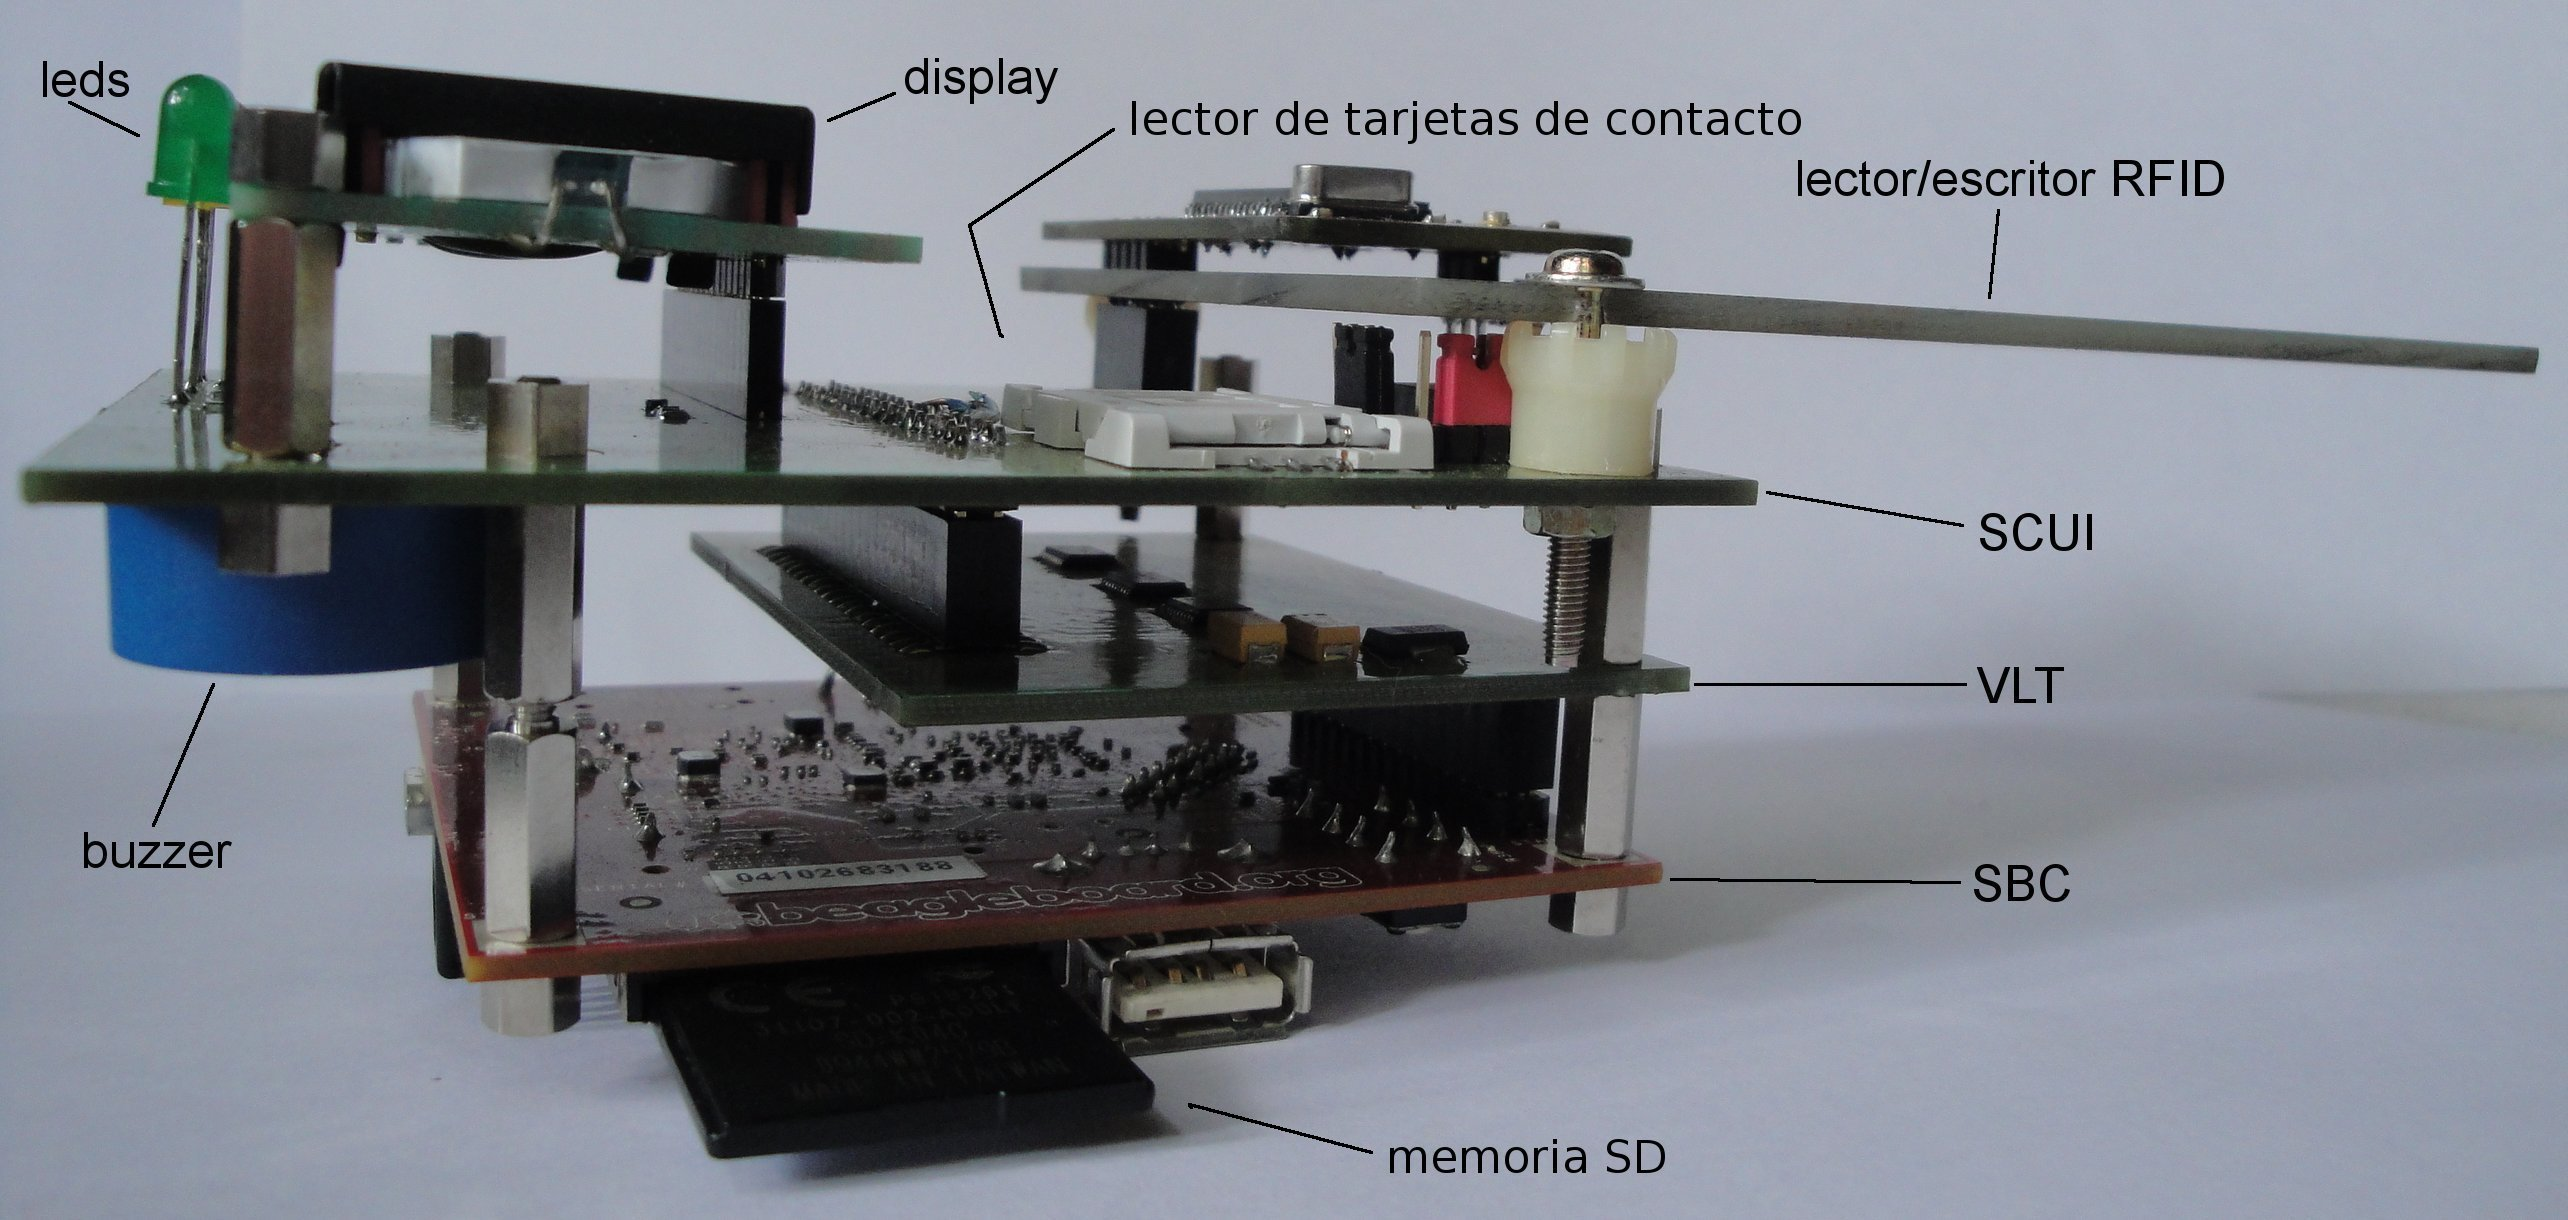
\includegraphics[scale=.15]{Imagenes/prototipo_s_nombres.jpg}
  \end{center}
  \caption{Vista general del prototipo}\label{prototipo} 
\end{figure}

\begin{figure}[H]
  \centering
  \subfigure[Vista anversa del prototipo]{\label{protoF}
  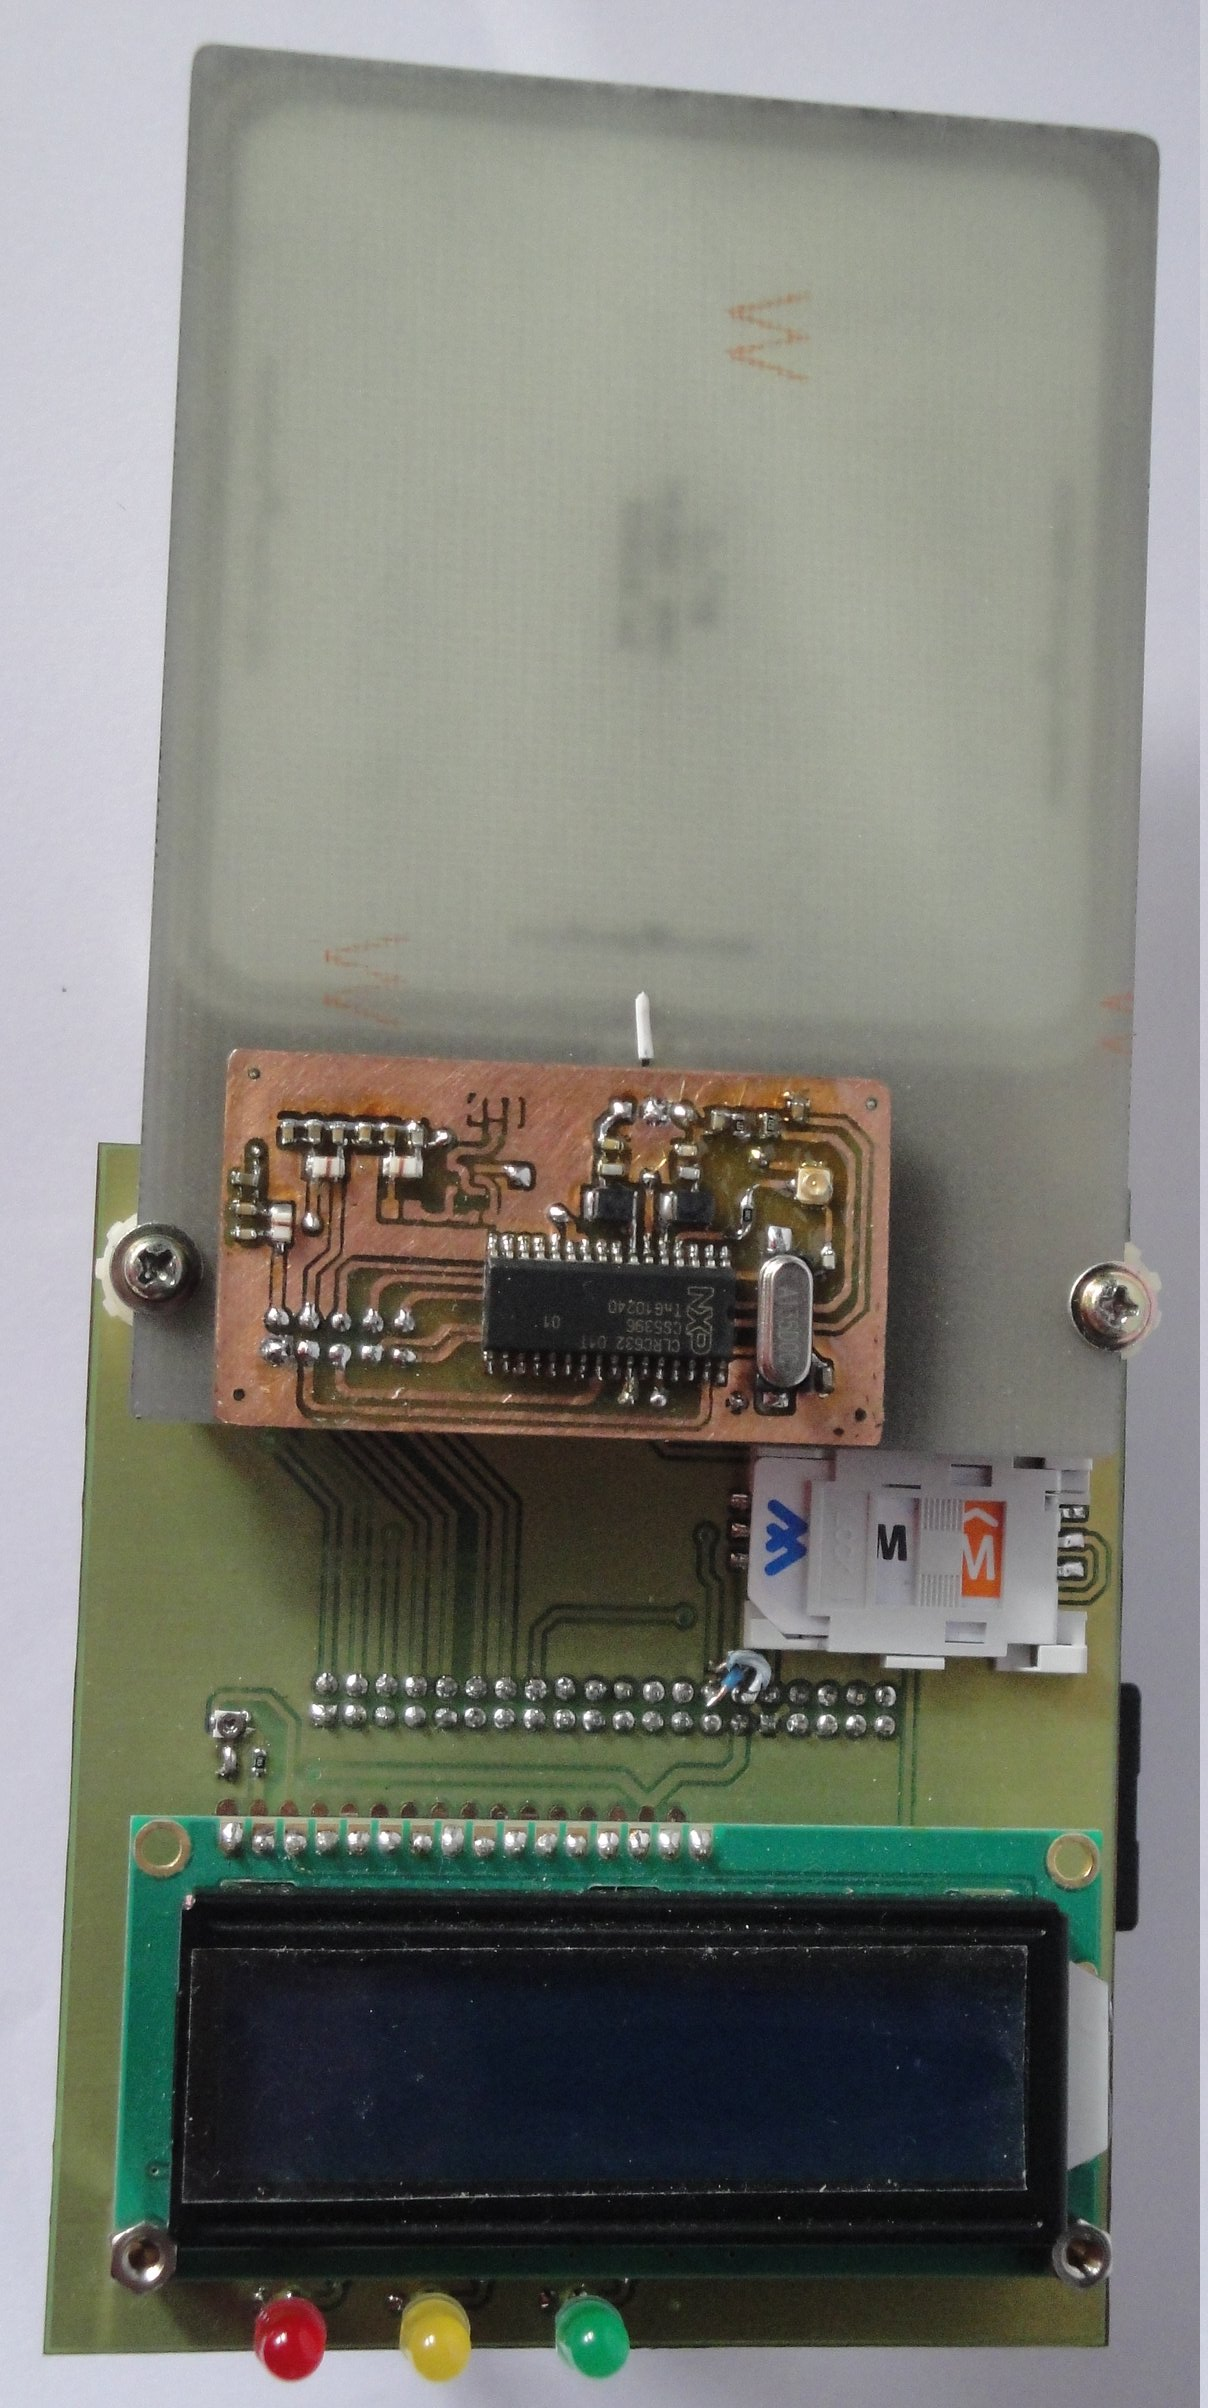
\includegraphics[scale=.13]{Imagenes/prototipo_f.jpg} } 
  \subfigure[Vista reversa del prototipo]{\label{protoB} 
  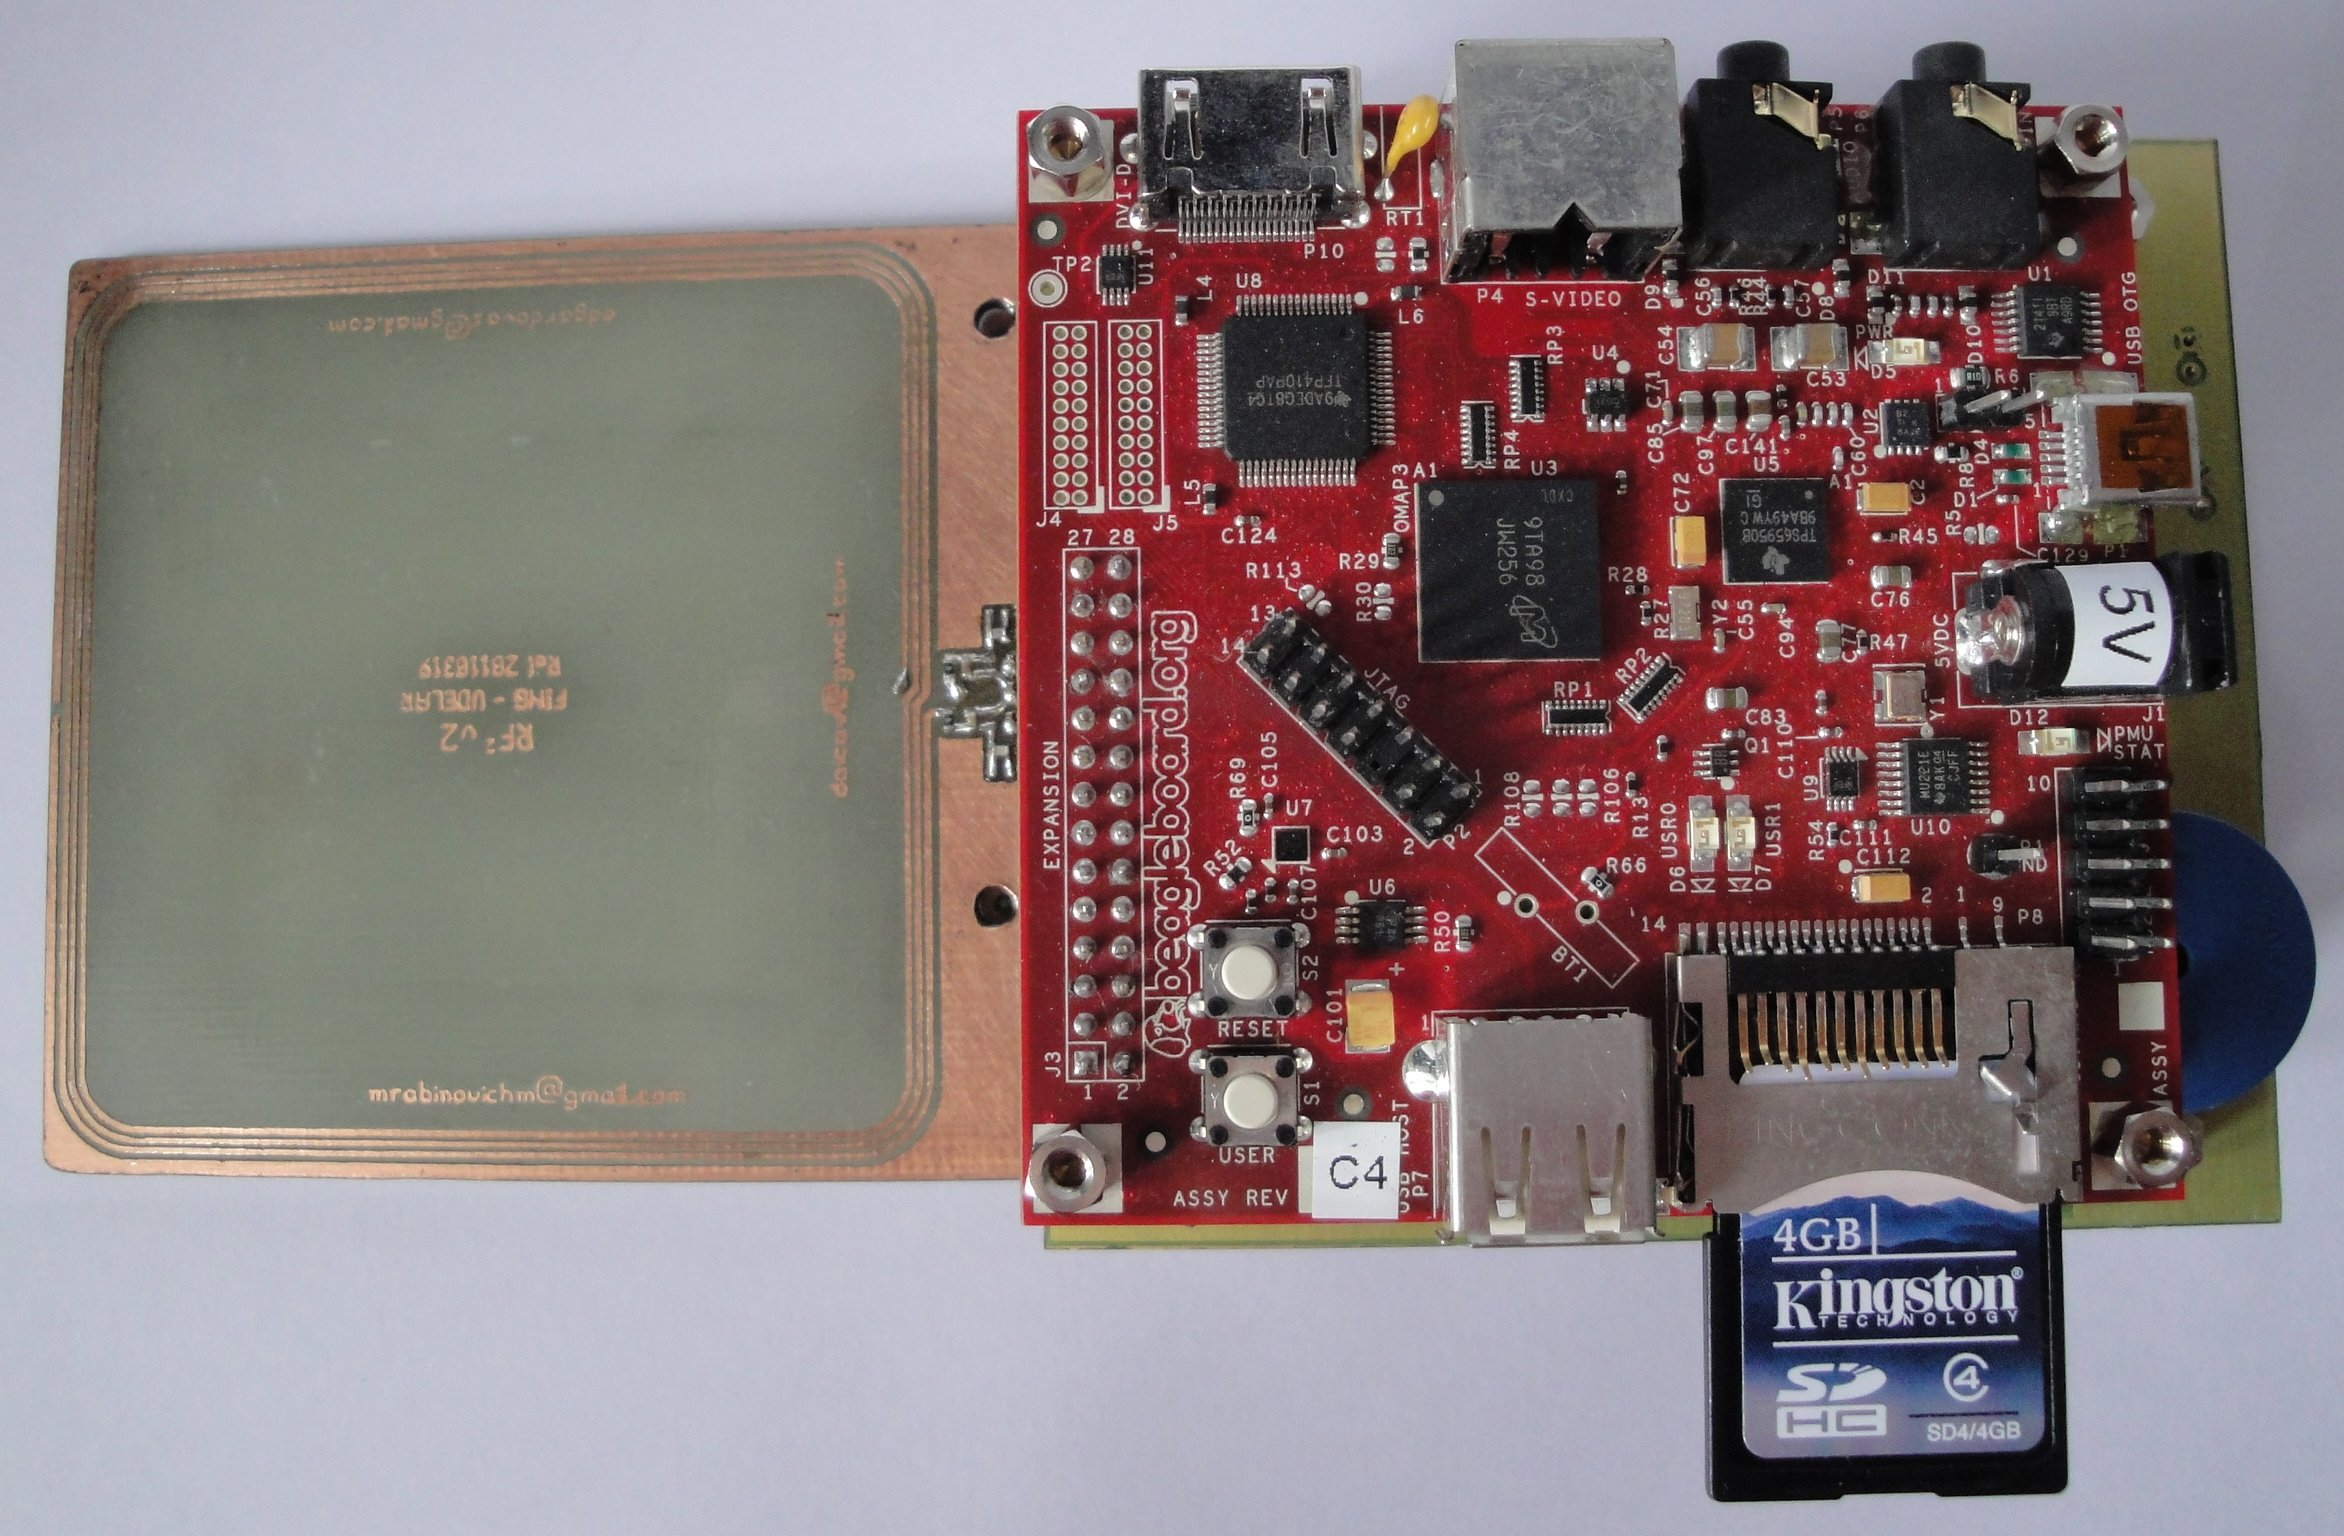
\includegraphics[scale=.13]{Imagenes/prototipo_b.jpg} }

  \caption{Vista anversa y reversa del prototipo}\label{protoFB}
\end{figure}

En cuanto al software, está basado en bibliotecas de código abierto que permiten desarrollar la aplicación que asegura el manejo del hardware y el funcionamiento de todo el sistema en conjunto.

\bigskip
Debe indicarse que las funcionalidades que brinda el módulo de seguridad no son usadas en la aplicación final. Si bien el hardware que compone el lector/escritor de tarjetas de contacto está operativo, ya que fue probado con una pequeña aplicación que permite enviar comandos APDU a la tarjeta de seguridad, no fue posible integrar este lector/escritor a la lista de dispositivos compatibles con la biblioteca PCSC-Lite.

En cuanto a la comunicación con el servidor indicado en el bloque de la figura \ref{HW_gral}, no está implementada por quedar fuera del alcance del proyecto.

\section{Funcionamiento general del prototipo}
Una vez que el prototipo RF$^{2}$ se encuentra operativo, el dispositivo despliega en el display el mensaje “Aproxime su tarjeta”, permaneciendo en dicho estado hasta que algún usuario acerque una tarjeta al lector/escritor RFID. 
En la primera transacción entre lector y tarjeta se obtiene el identificador único (UID) de ésta última, que será enviado al módulo de seguridad SAM (previa autenticación exitosa), para que a partir de éste, se generen las claves de acceso que permitan la lectura y escritura de la tarjeta RFID.
Mientras se lleva a cabo la operación, se despliega en el display el mensaje, “No retire su tarjeta” a la vez que el led amarillo es encendido para indicar precaución ya que se están procesando datos.
La siguiente acción a llevar a cabo es verificar que la tarjeta del usuario tenga saldo pendiente de acreditar, en caso afirmativo se indica al usuario el saldo a acreditar a través del display con el mensaje “Saldo a acreditar \$...”. Si todo fue exitoso, se borra el saldo transferido de la lista de saldos pendientes a acreditar para que no se transfiera saldo indefinidas veces.
A continuación se despliega en el display el nuevo monto almacenado en la tarjeta, “Su saldo es de \$...”, se enciende el led verde y se emite un pitido mediante el buzzer en señal que la operación fue satisfactoria.
Por último se muestran en el display los mensajes “Transacción finalizada”, “Gracias” y vuelve al inicio para comenzar un nuevo ciclo.

En caso que la tarjeta no tuviera saldo pendiente de acreditar, el prototipo RF$^{2}$ funciona en modo consulta y despliega en el display el saldo disponible en la tarjeta, “Su saldo es de \$...”, encendiendo el led verde y emitiendo un pitido, seguido de los mensajes “Transacción finalizada”, “Gracias” y vuelve al inicio para comenzar un nuevo ciclo.

En caso de ocurrir un error durante alguno de los pasos anteriores, ya sea porque
el usuario retiró la tarjeta en un momento inadecuado, o simplemente porque el prototipo RF$^{2}$
no logró leer o escribir la tarjeta en forma correcta, se enciende el led rojo, se emite un
doble pitido mediante el buzzer, y el display muestra el mensaje “Error, vuelva a intentarlo”,
acto seguido el ciclo vuelve a comenzar. 

\begin{figure}[H]
\centering
  \begin{center}
   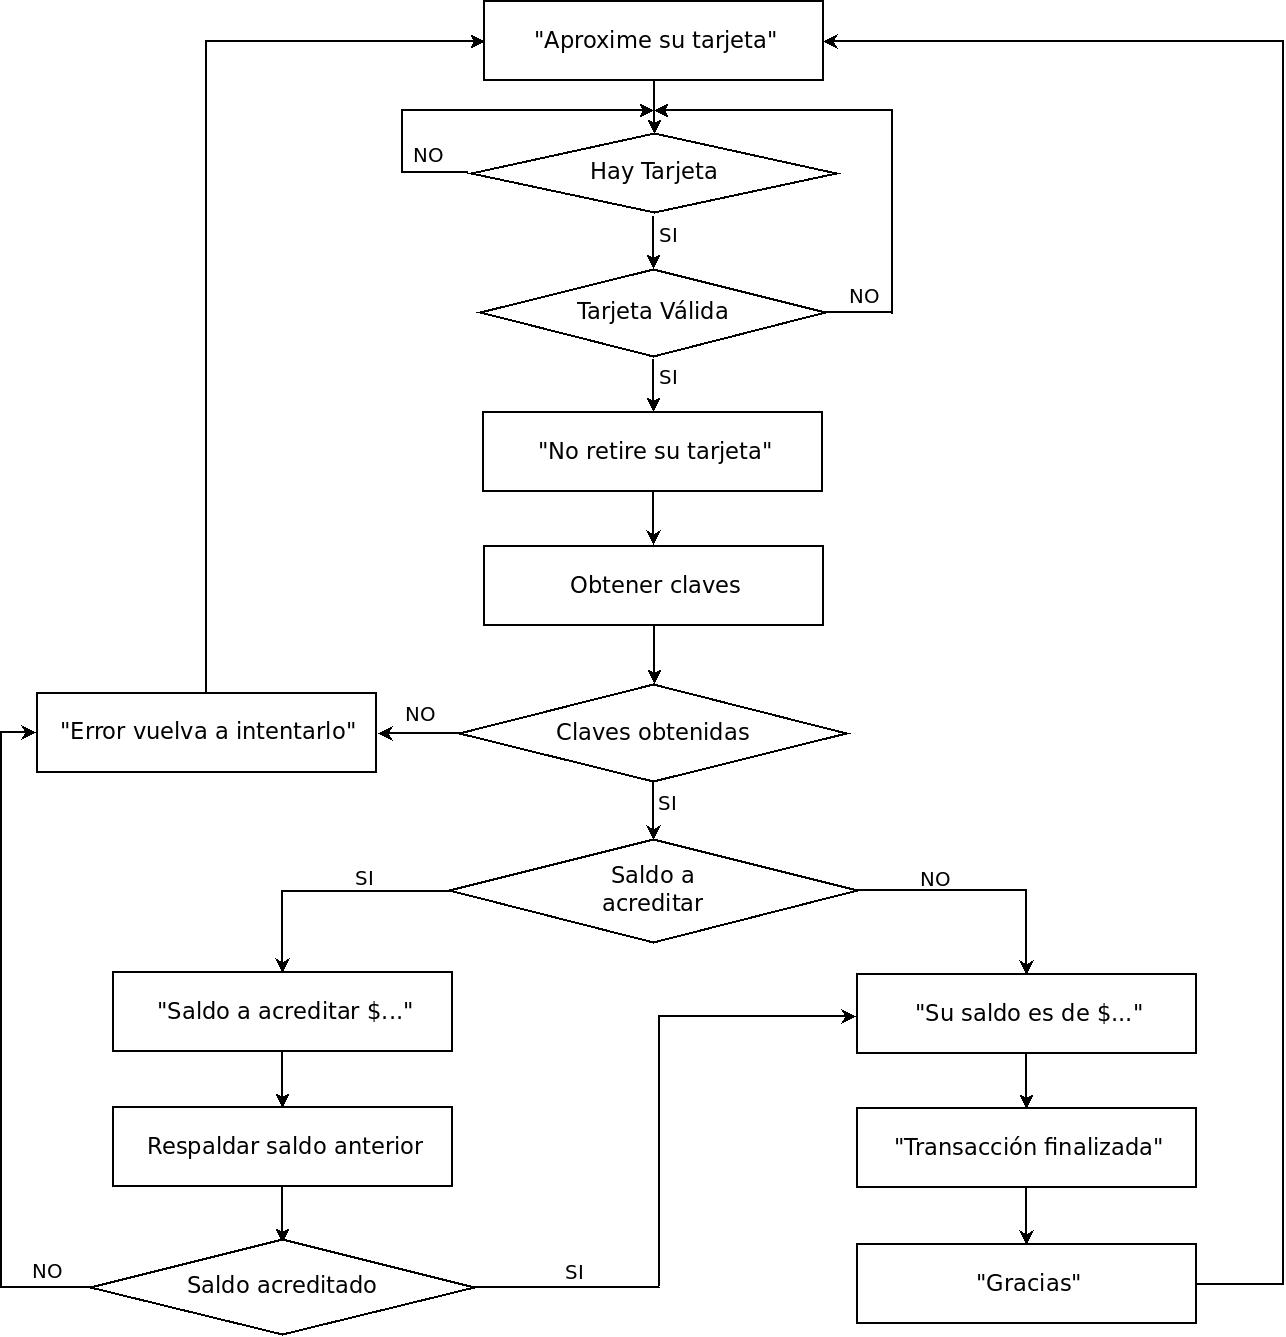
\includegraphics[scale=.35]{Imagenes/flujo.jpg}
  \end{center}
  \caption{Diagrama de flujo}\label{Fig:HW} 
\end{figure}